\chapter{Proposed Design}

The project will be split into three views, the first, which will be similar to the wireframe in figure \ref{fig:view1} is a selection screen with a text area, where the user can select tags to search by inputting them.

\begin{figure}
	\caption[Screenshot of the Category Selection View]{Screenshot of the category selection view, where the user inputs the category of article they want to read, as well as their experience level.}
	\label{fig:view1}
	\begin{center}
	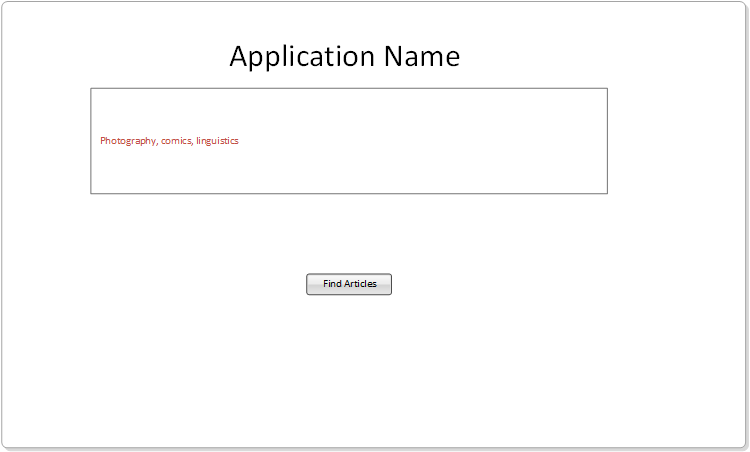
\includegraphics[width=\textwidth]{Graphics/View1}
	\end{center}
\end{figure}

Once the user inputs their preferred categories, the application takes those categories and finds relevant L2 articles by looking at articles on various sites, it then takes those articles and displays the title of each article, similar to view shown in figure \ref{fig:view2}

\begin{figure}
	\caption[Screenshot of the Article Selection View]{An example of the article selection view, here the user is shown a list of articles in their selected category as well as the difficulty rating for each article. They then go on to select an article from the list.}
	\label{fig:view2}
	\begin{center}
	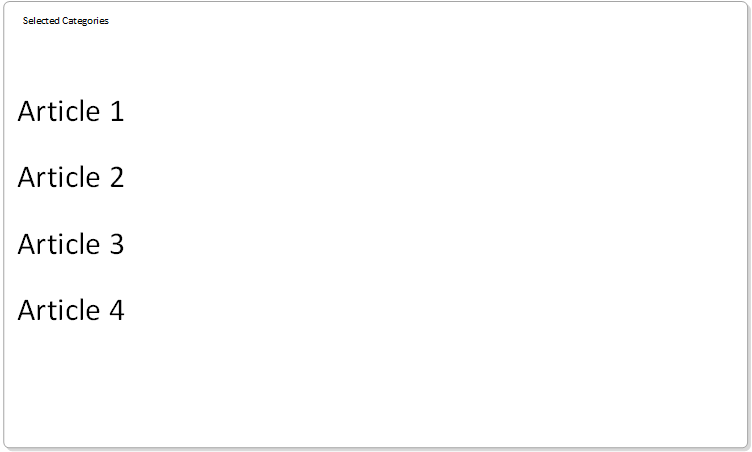
\includegraphics[width=\textwidth]{Graphics/View2}
\end{center}
\end{figure}

From the view shown in figure \ref{fig:view2} the user can select an article, once they do so, the application will download and parse the article, displaying it to the user, similar to the view in figure \ref{fig:view3}.

\begin{figure}
	\caption[Screenshot of the Article Reading View]{The article reading view, where the user can read the contents of their selected article. To the left of the article content is a button taking them back to article selection view and to the right is the gloss column, which contains a prompt telling the user click on articles. }
	\label{fig:view3}
	\begin{center}
	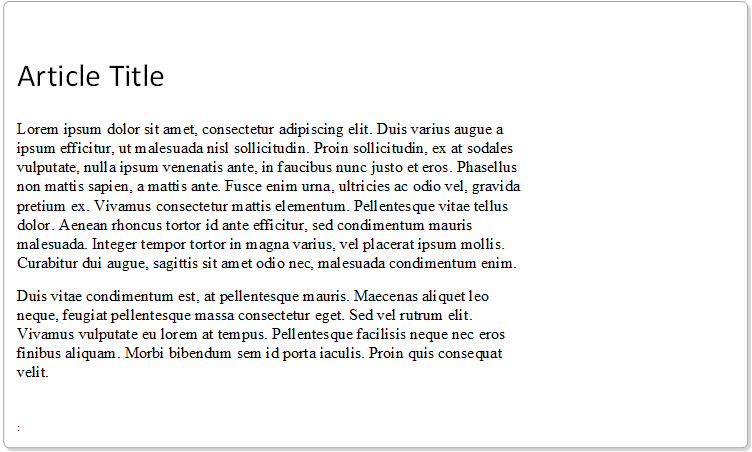
\includegraphics[width=0.7\textwidth]{Graphics/View3}
\end{center}
\end{figure}

from figure \ref{fig:view3} the user can select a word in the article, this action will send a request to the server for a gloss. The server will then look up translations of the word, along with grammatical information for the word, it will then serve the content, properly formatted, to the user, in a marginal gloss looking similar to the view in figure \ref{fig:view4}.

\begin{figure}
	\caption[Screenshot of the Article Reading View with Gloss]{Another screenshot of the article reading view, this time with a gloss entry in the margin.}
	\label{fig:view4}
	\begin{center}
	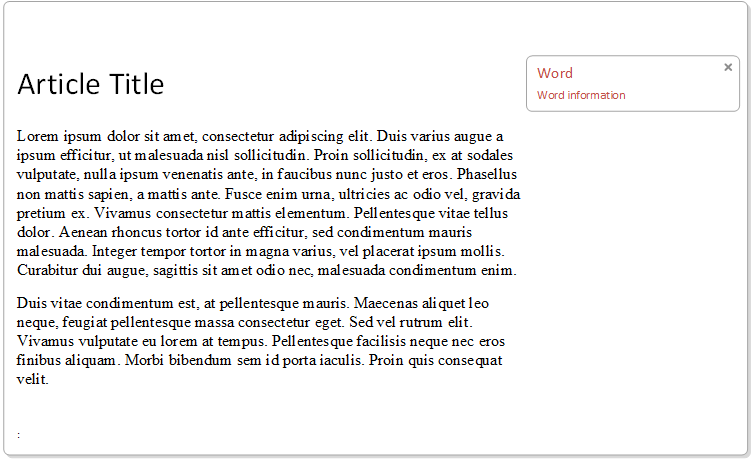
\includegraphics[width=\textwidth]{Graphics/View4}
\end{center}
\end{figure}

The whole systems process is illustrated in figure \ref{fig:sf}.
	
\begin{figure}
	\caption{Wireframe Mockup of the Category Input View}
	\label{fig:sf}
	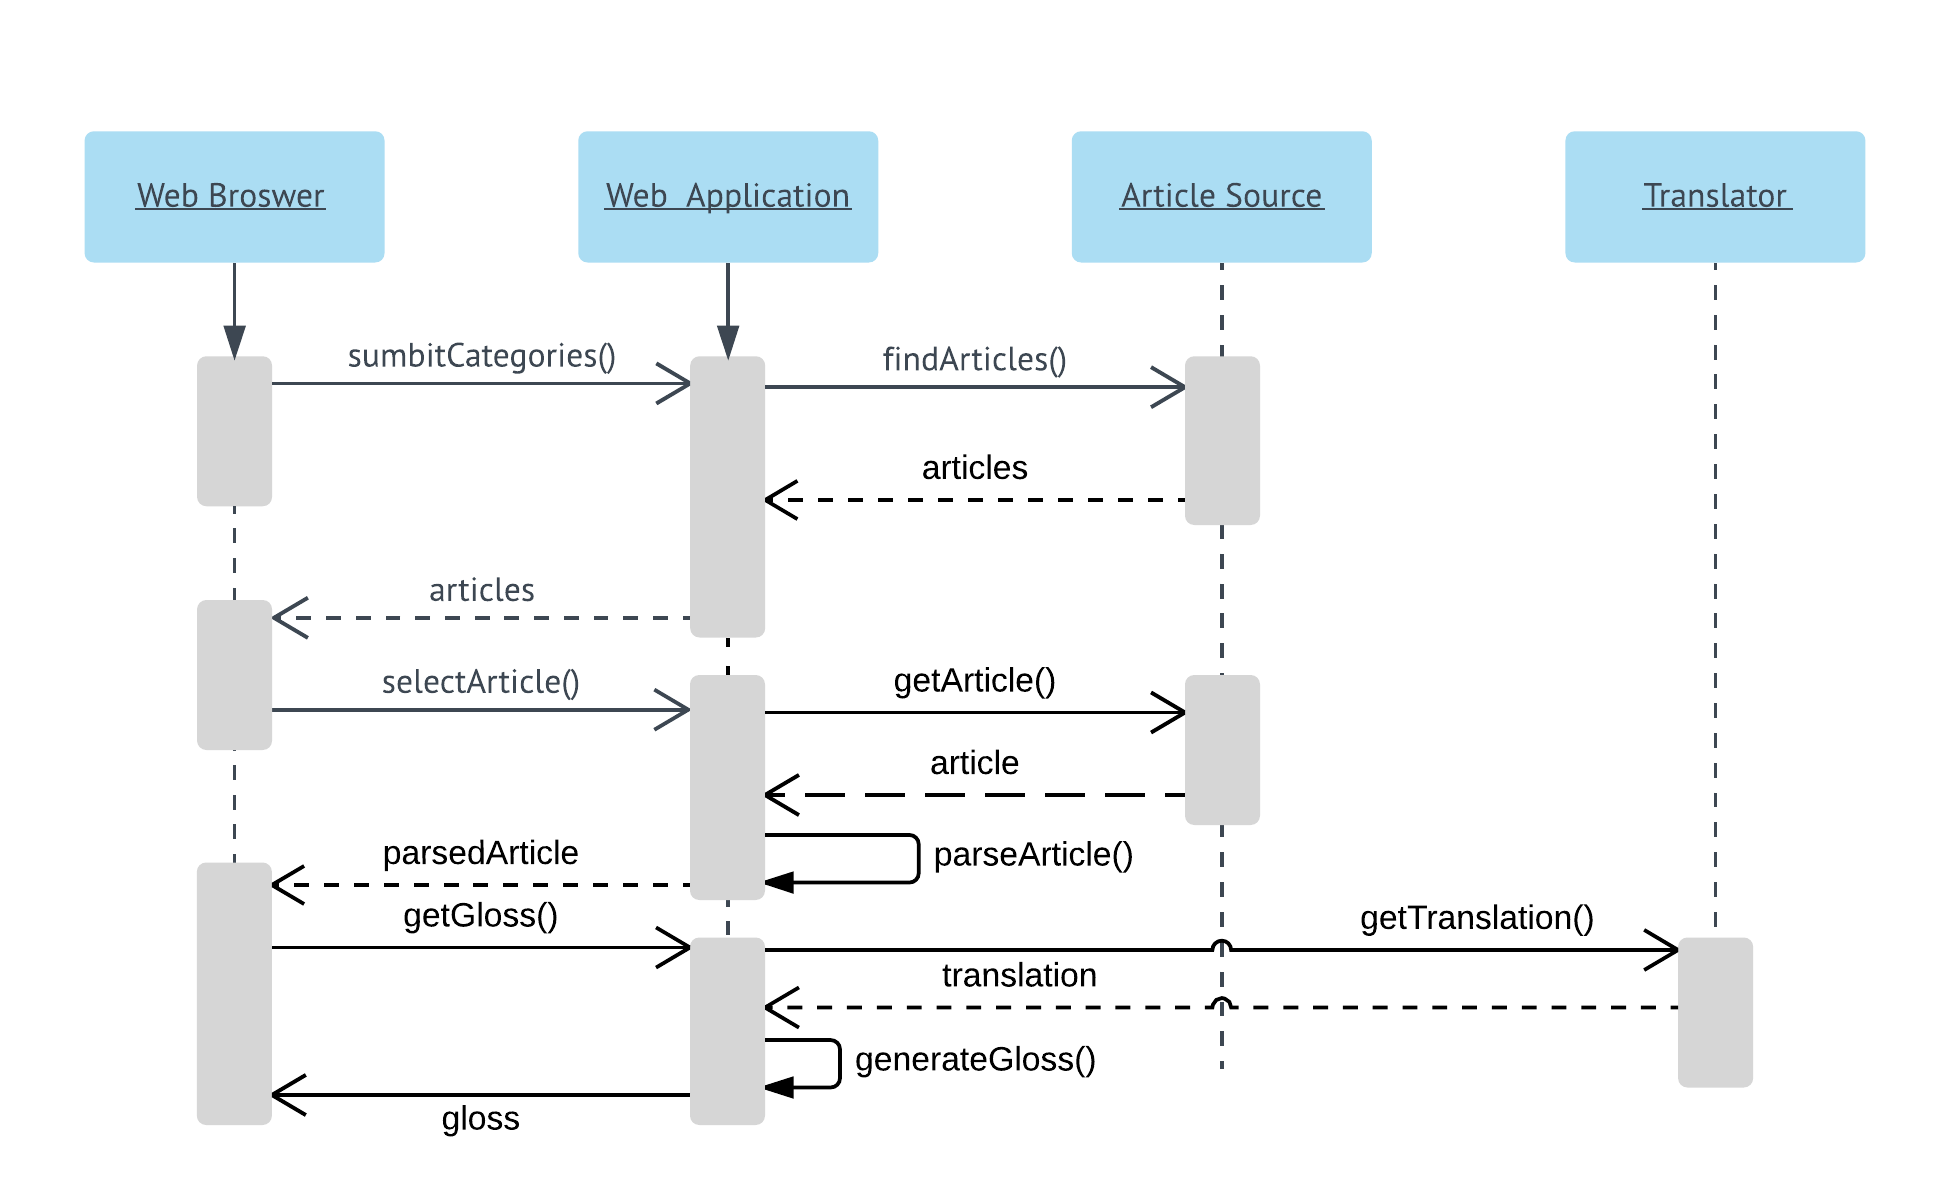
\includegraphics[width=\textwidth]{Graphics/SystemsFlow}
\end{figure}

